%\hypertarget{actividades}{} 

%\section*{\centering \textbf{Actividades}}
%\addcontentsline{toc}{section}
%{\protect \numberline{I. }Actividades} 
% \rule{\textwidth}{0.4pt} % Línea horizontal 
%\label{intro}
%\input{Components/Activities}


\textbf{\textit{Abstract}} - Este artículo presenta la planificación y desarrollo de un sistema de registro de actividades para ejecutivos en caja Incasur. El objetivo principal es mejorar la eficiencia y organización de las tareas diarias, permitiendo a los ejecutivos llevar un control de sus actividades, adicionalmente estableciendo dashboards tanto para el ejecutivo como el gerente, y propuesta de innovación se establece aplicar tecnología de visualización de datos y análisis de rendimiento usando un modelo de machine learning. Se describen las funcionalidades clave del sistema, así como la metodología utilizada para su implementación. Además, se discuten los beneficios esperados y las posibles mejoras futuras.

Todos los códigos fuente, se encuentran dentro del repositorio del proyecto, el cual se encuentra disponible en GitHub aplicando las licencias respectivas para su uso: \url{https://github.com/ArelyX1/Caja-Incasur-Activities-Register-System/tree/main}.
\vspace{0.5em}

\textbf{\textit{Index Terms}} - Caja Incasur, registro de actividades, ejecutivos, eficiencia, organización, visualización de datos, análisis de rendimiento, machine learning.

\section{Introducción}
\label{intro}
aaaaaaaaaaaaaaaaa


\section{Diseño del sistema}
\label{design}
EjemploEjemploEjemploEjemploEjemploEjemploEjemploEjemploEjemploEjemploEjemploEjemploEjemploEjemploEjemploEjemploEjemploEjemploEjemploEjemploEjemploEjemploEjemploEjemploEjemploEjemploEjemploEjemploEjemploEjemploEjemploEjemploEjemploEjemploEjemploEjemploEjemploEjemploEjemploEjemploEjemploEjemploEjemploEjemploEjemploEjemploEjemploEjemploEjemploEjemploEjemploEjemploEjemploEjemploEjemploEjemploEjemploEjemploEjemploEjemploEjemploEjemploEjemploEjemploEjemploEjemploEjemploEjemploEjemploEjemploEjemploEjemploEjemploEjemploEjemploEjemploEjemploEjemploEjemploEjemploEjemploEjemploEjemploEjemploEjemploEjemploEjemploEjemploEjemploEjemploEjemploEjemploEjemploEjemploEjemploEjemploEjemploEjemploEjemploEjemploEjemploEjemploEjemploEjemploEjemploEjemploEjemploEjemploEjemploEjemploEjemploEjemploEjemploEjemploEjemploEjemploEjemploEjemplo


\clearpage
\newpage

\begin{strip}
    \centering
    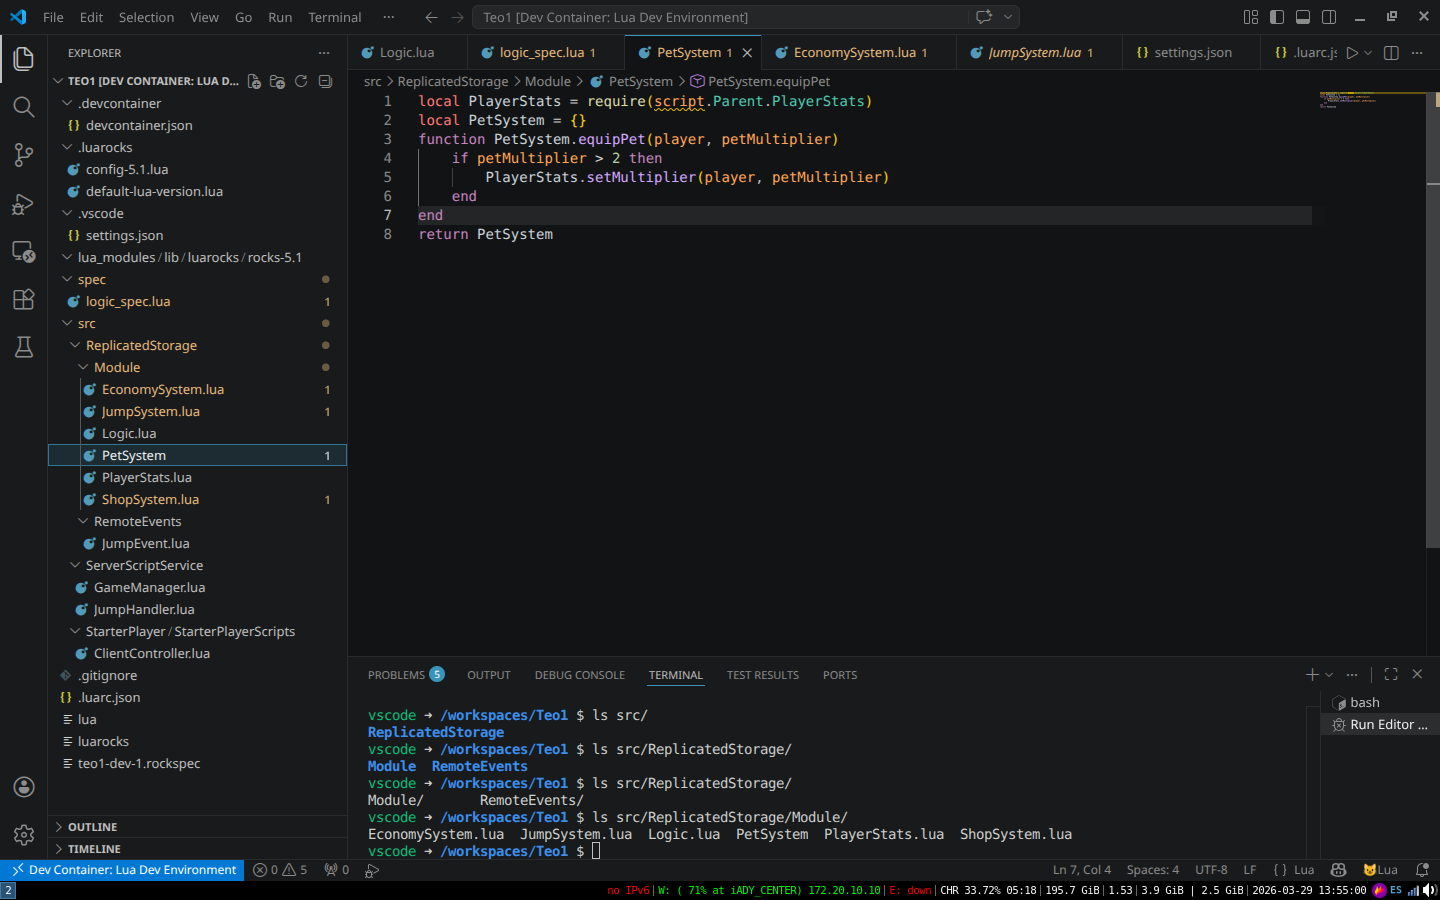
\includegraphics[width=1\textwidth]{media/FigGeneral/1.png}
    \captionof{figure}{Workspace de Visual Studio Code con Dev Containers}
    \label{fig:workflow_isometrico}
\end{strip}

Ejemplo de cita de imagen \cref{fig:workflow_isometrico},EjemploEjemploEjemploEjemploEjemploEjemploEjemploEjemploEjemploEjemploEjemploEjemploEjemploEjemploEjemploEjemploEjemploEjemploEjemploEjemploEjemploEjemploEjemploEjemploEjemploEjemploEjemploEjemploEjemploEjemploEjemploEjemploEjemploEjemploEjemploEjemploEjemploEjemploEjemploEjemploEjemploEjemploEjemploEjemploEjemploEjemploEjemploEjemploEjemploEjemploEjemploEjemploEjemploEjemploEjemploEjemploEjemploEjemploEjemploEjemploEjemploEjemploEjemploEjemploEjemploEjemploEjemploEjemploEjemploEjemploEjemploEjemploEjemploEjemploEjemploEjemploEjemploEjemploEjemploEjemploEjemploEjemploEjemploEjemploEjemploEjemploEjemploEjemploEjemploEjemploEjemploEjemploEjemploEjemploEjemploEjemploEjemploEjemploEjemploEjemploEjemploEjemploEjemploEjemploEjemploEjemploEjemploEjemploEjemploEjemploEjemploEjemploEjemploEjemploEjemploEjemploEjemploEjemplo

EjemploEjemploEjemploEjemploEjemploEjemploEjemploEjemploEjemploEjemploEjemploEjemploEjemploEjemploEjemploEjemploEjemploEjemploEjemploEjemploEjemploEjemploEjemploEjemploEjemploEjemploEjemploEjemploEjemploEjemploEjemploEjemploEjemploEjemploEjemploEjemploEjemploEjemploEjemploEJ ejemplo 



EjemploEjemploEjemploEjemploEjemploEjemploEjemploEjemploEjemploEjemploEjemploEjemploEjemploEjemploEjemploEjemploEjemploEjemploEjemploEjemploEjemploEjemploEjemploEjemploEjemploEjemploEjemploEjemploEjemploEjemploEjemploEjemploEjemploEjemploEjemploEjemploEjemploEjemploEjemploEjemploEjemploEjemplo

\begin{table}[H]
\renewcommand{\arraystretch}{1.3} % Da un poco de aire a las filas
\caption{Resumen de Métricas de Rendimiento del Módulo PlayerStats}
\label{table_stats}
\centering
\begin{tabular}{l|ccc} % 'l' alineado a la izquierda, 'c' centrado
\toprule
\textbf{ID Test} & \textbf{Tiempo (ms)} & \textbf{Memoria (MB)} & \textbf{Estado} \\
\midrule
PS-001 & 12.5 & 4.2 & \textit{Passed} \\
PS-002 & 8.9  & 3.8 & \textit{Passed} \\
PS-003 & 45.2 & 12.1 & \textit{Warning} \\
PS-004 & 10.1 & 4.0 & \textit{Passed} \\
\bottomrule
\end{tabular}
\end{table}


Esto siempre se usa para que las imagenes que ocupen el ancho deben ser siempre lo primero en mostrar porque sino se malogra el formato



\clearpage
\newpage

\begin{strip}
    \vspace{0.5cm}

    \captionof{table}{Resumen de Métricas de Rendimiento del Módulo PlayerStats}
    \label{table_stats}
    % Asegúrate de que tabularx tenga el ancho y las columnas X
    \begin{tabularx}{\textwidth}{X c c c} 
        \toprule
        \textbf{ID Test} & \textbf{Tiempo (ms)} & \textbf{Memoria (MB)} & \textbf{Estado} \\ \midrule
        PS-001 & 12.5 & 4.2 & Passed \\
        PS-002 & 8.9  & 3.8 & Passed \\
        PS-003 & 45.2 & 12.1 & Warning \\
        PS-004 & 10.1 & 4.0 & Passed \\ \bottomrule
    \end{tabularx}
\end{strip}

EjemploEjemploEjemploEjemploEjemploEjemploEjemploEjemploEjemploEjemploEjemploEjemploEjemploEjemploEjemploEjemploEjemploEjemploEjemploEjemploEjemploEjemploEjemploEjemploEjemploEjemploEjemploEjemploEjemploEjemploEjemploEjemploEjemploEjemploEjemploEjemploEjemploEjemploEjemploEjemploEjemploEjemploEjemploEjemploEjemploEjemploEjemploEjemploEjemploEjemploEjemploEjemploEjemploEjemploEjemploEjemploEjemploEjemploEjemploEjemploEjemploEjemploEjemploEjemploEjemploEjemploEjemploEjemploEjemploEjemploEjemploEjemploEjemploEjemploEjemploEjemploEjemploEjemploEjemploEjemploEjemploEjemploEjemploEjemploEjemploEjemploEjemploEjemploEjemploEjemploEjemploEjemploEjemploEjemploEjemploEjemploEjemploEjemploEjemploEjemploEjemploEjemploEjemploEjemploEjemploEjemploEjemploEjemploEjemploEjemploEjemploEjemploEjemploEjemploEjemploEjemploEjemploEjemplo


\begin{figure}[H]
    \centering
    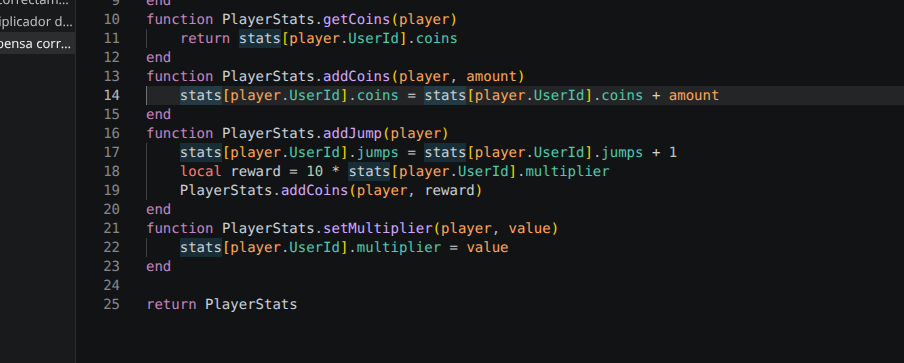
\includegraphics[width=\columnwidth]{media/FigGeneral/3fixbbug.png}
    \captionof{figure}{Solución del bug en el módulo PlayerStats}
    \label{fig:fix1}
\end{figure}

EjemploEjemploEjemploEjemploEjemploEjemploEjemploEjemploEjemploEjemploEjemploEjemploEjemploEjemploEjemploEjemploEjemploEjemploEjemploEjemploEjemploEjemploEjemploEjemploEjemploEjemploEjemploEjemploEjemploEjemploEjemploEjemploEjemploEjemploEjemploEjemploEjemploEjemploEjemploEjemploEjemploEjemploEjemploEjemploEjemploEjemploEjemploEjemploEjemploEjemploEjemploEjemploEjemploEjemploEjemploEjemploEjemploEjemploEjemploEjemploEjemploEjemploEjemploEjemploEjemploEjemploEjemploEjemploEjemploEjemploEjemploEjemploEjemploEjemploEjemploEjemploEjemploEjemploEjemploEjemploEjemploEjemploEjemploEjemploEjemploEjemploEjemploEjemploEjemploEjemploEjemploEjemploEjemploEjemploEjemploEjemploEjemploEjemploEjemploEjemploEjemploEjemploEjemploEjemploEjemploEjemploEjemploEjemploEjemploEjemploEjemploEjemploEjemploEjemploEjemploEjemploEjemploEjemplo




\section{Desarrollo del sistema}
\label{development}
\input{Components/development.tex}


\section{Resultados y discusión}
\label{results}
\input{Components/results.tex}



\section{Conclusiones}
\label{conclusiones}

\begin{enumerate}
    \item conclusión 1
    \item conclusión 2
\end{enumerate}